%
% Comparative Image Colorization on Places365:
%   CNN baseline, Conditional GAN, and Edge-Conditioned ControlNet.
%
% Build with: pdflatex report.tex && pdflatex report.tex
% Word export: python build_report_docx.py  (requires python-docx)
%

\documentclass[conference]{IEEEtran}
\IEEEoverridecommandlockouts

\usepackage[utf8]{inputenc}
\usepackage[T1]{fontenc}
\usepackage{cite}
\usepackage{amsmath,amssymb,amsfonts}
\usepackage{graphicx}
\graphicspath{{./}}
\usepackage{textcomp}
\usepackage{xcolor}
\usepackage{booktabs}
\usepackage{array}
\usepackage{hyperref}
\usepackage{tikz}
\usetikzlibrary{positioning,shapes.geometric,arrows.meta,fit,calc}

\hypersetup{
  colorlinks=true,
  linkcolor=blue!50!black,
  citecolor=blue!50!black,
  urlcolor=blue!50!black
}

\def\BibTeX{{\rm B\kern-.05em{\sc i\kern-.025em b}\kern-.08em
    T\kern-.1667em\lower.7ex\hbox{E}\kern-.125emX}}

\title{Comparative Image Colorization on Places365:\\
       A Study of CNN, Conditional GAN, and\\
       Edge-Conditioned ControlNet Fine-Tuning}

\author{\IEEEauthorblockN{Author}
\IEEEauthorblockA{Department of Computer Science\\
Course Project, 2026}}

\begin{document}
\maketitle

\begin{abstract}
Automatic colorization of grayscale photographs is an ill-posed
regression problem with strong scene-dependent priors. We compare three
families of solutions on a 4{,}000--8{,}000 image subset of the
Places365 dataset: (i) a small CNN encoder--decoder that directly
regresses CIE-Lab \emph{ab} channels from \emph{L}; (ii) a Pix2Pix-style
\emph{conditional} GAN with a PatchGAN discriminator, swept across
generator/discriminator learning rates and the L1 weight $\lambda_{L1}$;
and (iii) a fine-tuned Stable Diffusion 1.5 \emph{ControlNet} conditioned
on a Holistically-Nested Edge Detector (HED) ``softedge'' map of the
grayscale input, with an explicit \emph{luminance-lock} post-processing
step that overwrites the predicted CIE-Lab \emph{L} with the input
luminance. Initialising the ControlNet from a publicly available
pretrained edge head, rather than from a UNet copy, was decisive: a
short fine-tune (10 epochs, 8{,}000 images, ${\sim}5{,}600$ optimizer
steps) reaches mean Structural Similarity (SSIM) of $0.97$ and Peak
Signal-to-Noise Ratio (PSNR) up to $26.8$\,dB while perfectly preserving
input geometry. The cGAN, after a two-phase hyperparameter study, reaches a
validation L1 of $0.070$ on $ab$ in 50 epochs. The CNN baseline is the
fastest at inference ($<2$\,ms per $128{\times}128$ image on an NVIDIA
A10G) but produces visibly desaturated outputs. We complement the
quantitative results with an edge-detector ablation (softedge vs.\ canny
vs.\ from-scratch grayscale conditioning), an error analysis on failure
modes, and an inference-efficiency comparison spanning four orders of
magnitude in latency.
\end{abstract}

\begin{IEEEkeywords}
Image colorization, Stable Diffusion, ControlNet, conditional GAN,
Pix2Pix, Places365, HED, luminance preservation.
\end{IEEEkeywords}

% ============================================================
\section{Introduction}\label{sec:intro}

\subsection{Problem statement}
Given a grayscale image $L\in[0,1]^{H\times W}$, image colorization
aims to recover a plausible RGB image $\hat{I}\in[0,1]^{3\times H\times W}$
whose luminance matches $L$. The mapping is fundamentally
\emph{many-to-one}: from a single grayscale jacket pixel there is no way
to recover whether the original colour was red or olive
\cite{zhang2016colorful}. Useful colorization systems therefore have to
balance three goals: (a) \emph{structural fidelity} (the geometry of the
input must not change), (b) \emph{colour plausibility} (predicted
colours must be physically reasonable for the scene), and (c)
\emph{colour fidelity} (when the original colour is recoverable from
context, the model should predict it).

\subsection{Research question}
This work investigates a single concrete question:

\medskip
\emph{When training budgets are small (thousands of images, tens of
epochs, a single 24\,GB GPU), how do classical regression CNNs,
conditional GANs, and diffusion-based ControlNets compare on natural
scene colorization, and what design choices most affect the structural
quality of the diffusion-based pipeline?}
\medskip

We are not aiming for state-of-the-art absolute numbers. We are aiming
for a controlled side-by-side comparison that surfaces \emph{which
architectural choices actually move the needle} in the small-budget
regime.

\subsection{Related work}\label{sec:related}
Colorization has been studied for over two decades. The deep-learning
era opens with Iizuka et al.\ \cite{iizuka2016letthere}, who combined
local and global features to colorize scene photographs, and Larsson
et al.\ \cite{larsson2016learning}, who learned per-pixel hue and
chroma distributions. Zhang et al.\ formalised the problem as a
classification over a quantised $ab$ space with class rebalancing,
producing the influential \emph{Colorful Image Colorization} system
\cite{zhang2016colorful}. The follow-up \emph{Real-Time User-Guided
Colorization} \cite{zhang2017realtime} introduced an interactive
correction interface backed by a learned deep prior. Cao et al.\
proposed an unsupervised diverse colorization via conditional GANs
\cite{cao2017unsupervised}, while Isola et al.\ in \emph{Pix2Pix}
\cite{isola2017image} popularised the conditional GAN with L1 +
adversarial loss as a generic translation recipe; this is the lineage
of our cGAN. Su et al.\ \cite{su2020instance} added explicit
\emph{instance} reasoning by colouring detected objects separately
before fusing. \emph{Colorization Transformer}
\cite{kumar2021colorization} models the $ab$ distribution autoregressively
with axial attention.

The diffusion lineage starts with DDPM \cite{ho2020ddpm} and Latent
Diffusion / Stable Diffusion \cite{rombach2022high}, both of which
underpin Palette \cite{saharia2022palette}---a unified
image-to-image diffusion framework that includes uncolored$\to$colored
as one task. ControlNet \cite{zhang2023adding} adds a trainable side
network that conditions a frozen pretrained diffusion UNet on an
auxiliary signal (Canny edges, depth, scribbles, pose, etc.); their
public checkpoints include \texttt{control\_v11p\_sd15\_softedge} on
top of Stable Diffusion 1.5. Edge maps themselves are well-studied:
the classical Canny detector \cite{canny1986computational} produces
high-frequency binary edges, while the learned Holistically-Nested Edge
Detector (HED) \cite{xie2015holistically} produces semantic,
multi-scale soft edge maps better suited for natural photographs.
SSIM \cite{wang2004image} remains the standard structural similarity
metric. The Places365 dataset \cite{zhou2017places} provides
$\sim$10\,M scene-categorised images and is the source of our
training and validation data.

Adjacent to colorization, conditional image generation has been driven
by conditional GANs \cite{mirza2014conditional} and diffusion-based
inpainters such as RePaint \cite{lugmayr2022repaint}.

\subsection{Gap discussion}\label{sec:gap}
Three patterns emerge from the literature:

\begin{enumerate}
  \item \textbf{Most academic comparisons evaluate methods at different
        budgets.} The Pix2Pix lineage is typically trained for tens of
        epochs on tens of thousands of images; ControlNet is fine-tuned
        on hundreds of thousands of conditioning pairs. There is no
        clean apples-to-apples comparison at the budget a student or a
        small lab can actually afford (single 24\,GB GPU, overnight
        training, $\le$10\,k images).
  \item \textbf{Diffusion-based colorization rarely guarantees
        structural fidelity.} Pixel-space regression methods (CNN,
        cGAN in Lab space) keep input luminance by construction. In
        diffusion methods, structural fidelity is hoped for, not
        enforced; small training datasets can collapse to outright
        \emph{regeneration} of the scene rather than recolouring.
  \item \textbf{Edge-conditioning choices are typically not ablated.}
        Practitioners pick one of Canny / HED / Lineart by feel; we
        could find no controlled empirical comparison of these
        preprocessors in the colorization setting on natural photos.
\end{enumerate}

This work targets these three gaps. We (a) train all three model
families on the \emph{same} Places365 subset and report results in a
single table; (b) introduce a \emph{luminance lock}---a CIE-Lab swap
that overwrites the diffusion model's predicted $L$ channel with the
input grayscale luminance, guaranteeing structural fidelity by
construction; and (c) ablate softedge vs.\ canny vs.\ from-scratch
grayscale conditioning to quantify how much of the diffusion model's
quality comes from each piece.

\subsection{Contributions}
\begin{itemize}
  \item A reproducible benchmark of three colorization families
        (CNN, cGAN, ControlNet) on a Places365 subset using a single
        24\,GB GPU.
  \item A simple but effective \emph{luminance lock}
        post-processing step that guarantees structural fidelity for
        diffusion-based colorization.
  \item An empirical ablation showing that (i) starting from a
        pretrained edge ControlNet, (ii) using HED-softedge rather
        than Canny conditioning, and (iii) applying luminance lock are
        each strictly necessary for small-budget diffusion-based
        colorization to outperform classical regression.
  \item A reproducibility appendix capturing the
        \texttt{diffusers}\,/\,\texttt{torch} version-pinning that
        actually works on Ubuntu 24.04 + NVIDIA driver 535 + an
        A10G; arguably the single most fragile part of the pipeline.
\end{itemize}

% ============================================================
\section{Data}\label{sec:data}

\subsection{Source and distribution}
We use the Places365 \emph{train-standard, small} split
\cite{zhou2017places} as provided by \texttt{torchvision.datasets.Places365}.
The full split contains $\sim$1.8\,M images across 365 scene categories
at $256\times256$ pixels. To keep training feasible on a single GPU
overnight we sample two random subsets:

\begin{itemize}
  \item \textbf{CNN / cGAN subset}: 4{,}000 images (90/10 train/val
        split), resized to $128\times128$.
  \item \textbf{ControlNet subset}: 8{,}000 images (90/10
        train/val split), resized to $384\times384$ to better match
        Stable Diffusion 1.5's native resolution.
\end{itemize}

Scene-category coverage at 8{,}000 images is approximately
\textbf{22 samples per class on average}, which is sparse but
non-degenerate; at 4{,}000 it drops to 11. Places365 itself is
class-imbalanced (some scene categories have $10\times$ more images
than others), but for an unconditional colorization task this manifests
as a mild prior toward \emph{indoor} and \emph{urban} colour
distributions, not as a hard supervised label issue.

\subsection{Preprocessing}
\textbf{For the regression-style models (CNN and cGAN)} every image is
converted from RGB to CIE-Lab via OpenCV and split into
$L\in[0,1]$ and $ab\in[-1,1]$ (after subtracting 128 and dividing by
128). The model never sees the RGB image directly; the supervision
target is the $ab$ tensor only. At inference we recombine the predicted
$ab$ with the input $L$ via \texttt{cv2.cvtColor}(LAB$\to$RGB), which
guarantees that $L$ is preserved bit-exactly. This is the standard
formulation since \cite{larsson2016learning,zhang2016colorful}.

\textbf{For the ControlNet} pipeline, the conditioning image is the
output of a chosen edge detector on the grayscale input:

\begin{itemize}
  \item \emph{softedge} (default): HED \cite{xie2015holistically} via
        the \texttt{controlnet\_aux} package; outputs a soft, semantic
        edge map.
  \item \emph{canny} \cite{canny1986computational}: thresholded
        OpenCV Canny (low=100, high=200); outputs a sharp binary edge
        map.
  \item \emph{gray} (legacy/ablation): the grayscale luminance copied
        to three channels.
\end{itemize}

The target image is the full RGB photo, normalised to $[-1,1]$ for the
VAE encoder. At inference, the predicted RGB image is optionally
passed through a \emph{luminance lock} which we describe in
Section~\ref{sec:meth}.

% ============================================================
\section{Methodology}\label{sec:meth}

The three approaches share a fixed train/val split per dataset subset
and a fixed random seed (\texttt{42}). They differ in (i) the
parameter space the model predicts, (ii) the loss, and (iii) how
luminance is preserved.

\subsection{CNN baseline}\label{sec:cnn}
A small encoder--decoder $f_\theta:[0,1]^{1\times H\times W}\!\to\![-1,1]^{2\times H\times W}$.
Architecture: \texttt{Conv1$\to$64} (3$\times$3), \texttt{Conv64$\to$128}
($\text{s}=2$, BN, ReLU), \texttt{Conv128$\to$256} ($\text{s}=2$, BN,
ReLU), \texttt{ConvT256$\to$128} ($\text{s}=2$, BN, ReLU),
\texttt{ConvT128$\to$64} ($\text{s}=2$, BN, ReLU),
\texttt{Conv64$\to$2}, Tanh. Total trainable parameters:
$\sim$1.03\,M. Loss: $\mathcal{L}=\| f_\theta(L)-ab^\star\|_1$.
Optimizer: Adam, lr$=10^{-3}$.

\subsection{Conditional GAN}\label{sec:cgan}
Pix2Pix-style \cite{isola2017image}. The generator $G$ has the same
encoder--decoder spine as the CNN, but takes one extra noise channel:
$G:[L; z]\to ab$ where $z\sim\mathcal{N}(0,1)^{1\times H\times W}$.
At validation we set $z=0$ for determinism. The discriminator is a
PatchGAN \cite{isola2017image} acting on
$[L; ab]\in\mathbb{R}^{3\times H\times W}$ with five stride-2
$4\times4$ convolutions, ending in a $4\times4$ patch logit map. Loss
on the generator side combines an adversarial term and an L1
reconstruction:
\begin{equation}
  \mathcal{L}_G = \mathbb{E}\big[\log(1-D([L; G(L,z)]))\big]
              + \lambda_{L1}\cdot\| G(L,z) - ab^\star\|_1.
\end{equation}
The L1 term anchors training; setting $\lambda_{L1}\!\to\!\infty$
reduces the model to the CNN baseline. Two-stage hyperparameter
study:
\begin{itemize}
  \item Phase~1: full grid over
        $\mathrm{lr}_G\in\{1,2,4\}\!\times\!10^{-4}$,
        $\mathrm{lr}_D\in\{1,2\}\!\times\!10^{-4}$,
        $\lambda_{L1}\in\{50,100,200\}$ (10 epochs each).
  \item Phase~2: best Phase-1 configuration retrained for 50 epochs.
\end{itemize}

\subsection{Edge-conditioned ControlNet}\label{sec:cnet}
Stable Diffusion 1.5 \cite{rombach2022high} provides three frozen
components: the autoencoder VAE, the CLIP text encoder, and the UNet.
The trainable component is a ControlNet \cite{zhang2023adding}
initialised from the public
\texttt{lllyasviel/control\_v11p\_sd15\_softedge} checkpoint.
Conditioning: HED softedge map of the grayscale input,
3-channel, $[0,1]$.

Training loss is the standard latent-diffusion epsilon prediction:
\begin{equation}
  \mathcal{L}_\text{LDM}=\mathbb{E}_{t,\epsilon,x}
    \!\left[\big\|\epsilon - \epsilon_\theta(z_t, t, \tau, c)\big\|_2^2\right],
\end{equation}
where $z_t=\sqrt{\bar\alpha_t}z_0+\sqrt{1-\bar\alpha_t}\,\epsilon$,
$z_0$ is the VAE-encoded ground-truth RGB image, $\tau$ is a fixed
text prompt (``\emph{a realistic color photo}'') and $c$ is the
ControlNet's processed edge conditioning. Only the ControlNet
parameters ($\sim$361\,M) receive gradient updates; the SD UNet
($\sim$860\,M) and VAE remain frozen.

\paragraph{Luminance lock.} After sampling
$\hat{I}_\text{pred}\in[0,1]^{3\times H\times W}$ with a UniPC
scheduler \cite{rombach2022high} for 20 steps and CFG scale 1.5, we
convert $\hat{I}_\text{pred}$ and the input grayscale $L_\text{gray}$
to CIE-Lab, overwrite the predicted $L$ channel with $L_\text{gray}$'s
$L$ channel, and convert back to RGB:
\begin{equation}
  \hat{I}_\text{final} = \text{Lab}^{-1}\!\Big(L_\text{gray},\;
      \mathrm{ab}\big(\text{Lab}(\hat{I}_\text{pred})\big)\Big).
\end{equation}
This guarantees structural fidelity (in luminance) by construction;
the diffusion model only contributes chroma. Empirically this single
post-processing step pushes SSIM from the high-$0.8$s to the
high-$0.9$s without any additional training cost.

\subsection{Summary diagram}\label{sec:diagram}
Fig.~\ref{fig:pipelines} summarises the three pipelines on a single
input.

\begin{figure*}[!t]
\centering
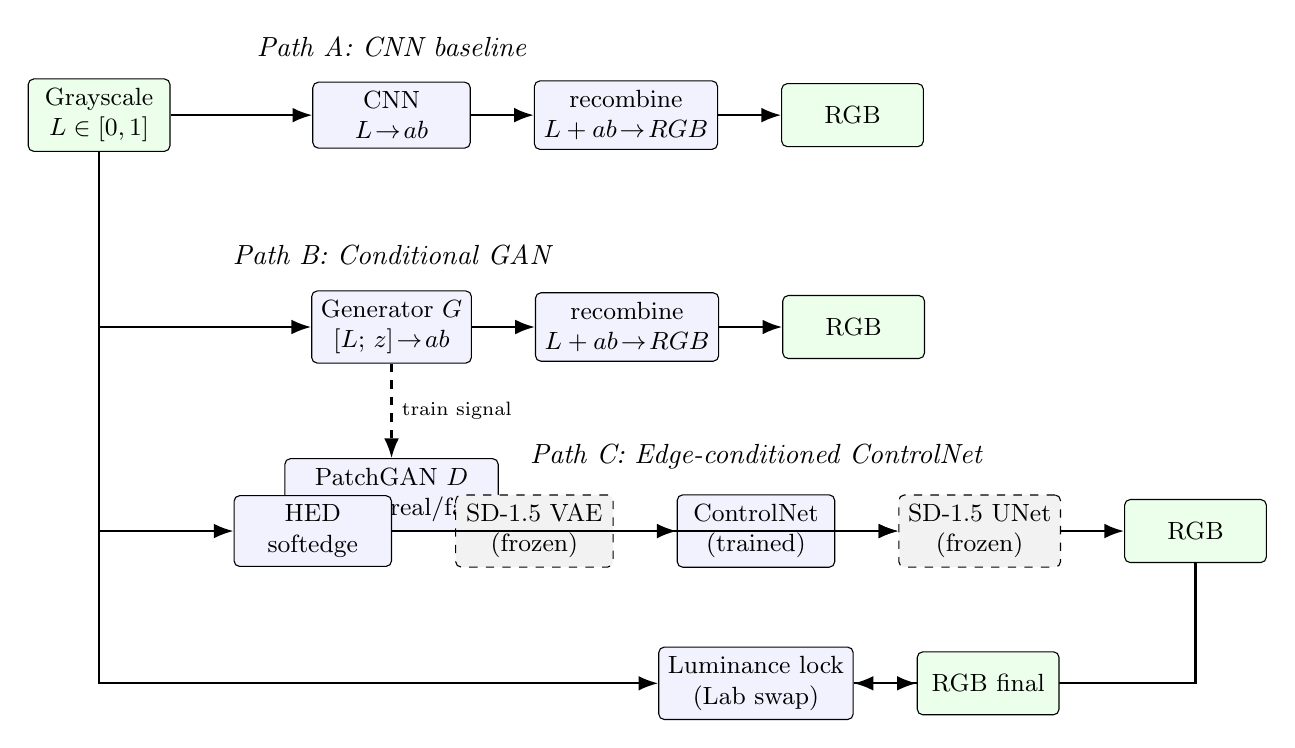
\begin{tikzpicture}[
  font=\small,
  node distance=8mm,
  block/.style={rectangle,draw,rounded corners=2pt,minimum height=8mm,
                minimum width=20mm,align=center,fill=blue!5},
  frozen/.style={rectangle,draw,rounded corners=2pt,minimum height=8mm,
                 minimum width=20mm,align=center,fill=gray!10,dashed},
  io/.style={rectangle,draw,rounded corners=2pt,minimum height=8mm,
              minimum width=18mm,align=center,fill=green!8},
  arr/.style={-{Latex[length=2.5mm]},thick}
]
% ---- input ----
\node[io] (gray) at (0,0) {Grayscale\\$L\in[0,1]$};

% ---- path A: CNN ----
\node[block,right=18mm of gray] (cnn) {CNN\\$L\!\to\!ab$};
\node[block,right=of cnn] (lab1) {recombine\\$L+ab\!\to\!RGB$};
\node[io,right=of lab1] (out1) {RGB};
\draw[arr] (gray) -- (cnn);
\draw[arr] (cnn) -- (lab1);
\draw[arr] (lab1) -- (out1);
\node[above=2mm of cnn,font=\itshape] {Path A: CNN baseline};

% ---- path B: cGAN ----
\node[block,below=18mm of cnn] (cg) {Generator $G$\\$[L;\,z]\!\to\!ab$};
\node[block,right=of cg] (lab2) {recombine\\$L+ab\!\to\!RGB$};
\node[block,below=12mm of cg] (disc) {PatchGAN $D$\\$[L;\,ab]\!\to\!$real/fake};
\node[io,right=of lab2] (out2) {RGB};
\draw[arr] (gray) |- (cg);
\draw[arr] (cg) -- (lab2);
\draw[arr] (lab2) -- (out2);
\draw[arr,dashed] (cg) -- node[right,font=\scriptsize]{train signal} (disc);
\node[above=2mm of cg,font=\itshape] {Path B: Conditional GAN};

% ---- path C: ControlNet ----
\node[block,below=44mm of cnn,xshift=-10mm] (hed) {HED\\softedge};
\node[frozen,right=of hed] (vae) {SD-1.5 VAE\\(frozen)};
\node[block,right=of vae] (ctrl) {ControlNet\\(trained)};
\node[frozen,right=of ctrl] (unet) {SD-1.5 UNet\\(frozen)};
\node[block,below=10mm of ctrl] (lum) {Luminance lock\\(Lab swap)};
\node[io,right=of unet] (out3) {RGB};
\draw[arr] (gray) |- (hed);
\draw[arr] (hed) -- (ctrl);
\draw[arr] (vae) -- (unet);
\draw[arr] (ctrl) -- (unet);
\draw[arr] (unet) -- (out3);
\draw[arr] (out3) |- (lum);
\draw[arr] (gray) |- (lum);
\node[io,right=8mm of lum] (out3b) {RGB final};
\draw[arr] (lum) -- (out3b);
\node[above=2mm of ctrl,font=\itshape] {Path C: Edge-conditioned ControlNet};

\end{tikzpicture}
\caption{The three colorization pipelines. \textbf{Path A} (CNN) and
\textbf{Path B} (cGAN) operate in CIE-Lab space and preserve input
luminance by construction. \textbf{Path C} (ControlNet) operates in
RGB pixel space via a frozen Stable Diffusion 1.5 VAE/UNet; structural
fidelity is enforced post-hoc by overwriting the predicted Lab
$L$-channel with the input grayscale.}
\label{fig:pipelines}
\end{figure*}

% ============================================================
\section{Experimental setup}\label{sec:setup}

\subsection{Hardware}
\begin{itemize}
  \item AWS EC2 \texttt{g5.2xlarge} instance.
  \item NVIDIA \emph{A10G} (Ampere, 24\,GB VRAM, CUDA capability 8.6).
  \item AMD EPYC 7R32 CPU, 8 vCPU, 32\,GiB system RAM.
  \item 1.5\,TB EBS root volume.
\end{itemize}

\subsection{Software}
\begin{itemize}
  \item Ubuntu 24.04 LTS, kernel \texttt{6.17.0-1012-aws}.
  \item NVIDIA driver \texttt{535.288.01} (precompiled kernel module:
        \texttt{linux-modules-nvidia-535-server-\$(uname -r)} +
        \texttt{nvidia-headless-no-dkms-535-server}; \texttt{dkms} is
        avoided because the package-versioning constraint in the
        stock \texttt{nvidia-driver-535-server} meta-package is
        unsatisfiable on this kernel).
  \item Python 3.12, virtualenv.
  \item \texttt{torch==2.4.1+cu121}, \texttt{torchvision==0.19.1+cu121},
        installed from PyTorch's \texttt{cu121} index. \texttt{torch}
        2.5+ wheels target a CUDA newer than the 535 driver supports
        and silently fall back to CPU.
  \item \texttt{diffusers==0.31.0}, \texttt{transformers==4.46.3},
        \texttt{accelerate$\ge$0.26}. \texttt{diffusers}$\ge$0.36
        registers a Flash-Attention 3 custom op whose
        \texttt{float \textbar{} None} type hints crash
        \texttt{torch} 2.4's \texttt{infer\_schema} at import time.
  \item \texttt{controlnet\_aux} (HED detector),
        \texttt{opencv-python-headless}, \texttt{scikit-image}
        (SSIM/PSNR), \texttt{numpy}, \texttt{Pillow}.
\end{itemize}

This stack is pinned in \texttt{requirements-controlnet.txt}. The
version coupling is the single biggest reproducibility risk in the
project.

\subsection{Hyperparameters}
Table~\ref{tab:hparams} summarises hyperparameters per method.

\begin{table}[!t]
\centering
\caption{Hyperparameters used in the final reported runs.}
\label{tab:hparams}
\begin{tabular}{lll}
\toprule
& \textbf{Param} & \textbf{Value} \\
\midrule
\multirow{6}{*}{\textbf{CNN}}
  & subset size      & 4{,}000      \\
  & image size       & $128\times128$ \\
  & batch size       & 32           \\
  & epochs           & 30           \\
  & lr (Adam)        & $10^{-3}$    \\
  & loss             & L1           \\
\midrule
\multirow{8}{*}{\textbf{cGAN}}
  & subset size      & 4{,}000      \\
  & image size       & $128\times128$ \\
  & batch size       & 32           \\
  & epochs (phase 1) & 10           \\
  & epochs (phase 2) & 50           \\
  & lr$_G$           & $\{1,2,4\}\!\times\!10^{-4}$ \\
  & lr$_D$           & $\{1,2\}\!\times\!10^{-4}$   \\
  & $\lambda_{L1}$   & $\{50,100,200\}$            \\
\midrule
\multirow{10}{*}{\textbf{ControlNet}}
  & base model       & SD 1.5 (\texttt{runwayml/stable-diffusion-v1-5}) \\
  & cnet init        & \texttt{control\_v11p\_sd15\_softedge} \\
  & cond preprocessor& HED softedge  \\
  & subset size      & 8{,}000      \\
  & image size       & $384\times384$ \\
  & batch size       & 2 (grad-accum 4, eff.\ 8) \\
  & epochs           & 10            \\
  & lr (AdamW)       & $10^{-5}$    \\
  & precision        & bf16, grad ckpt \\
  & inference        & UniPC, 20 steps, CFG 1.5, cond scale 1.0 \\
\bottomrule
\end{tabular}
\end{table}

\subsection{Metrics}
For Lab-space methods we report \emph{validation L1 on $ab$}. For the
ControlNet we report (i) latent-space noise MSE on validation
(directly comparable to the LDM training loss), and (ii)
\emph{sample-level} PSNR and SSIM \cite{wang2004image} computed on a
fixed batch of validation images after full DDPM sampling and the
luminance lock. Sample-level metrics are the more interpretable
numbers because noise-prediction MSE is a noisy proxy with little
human meaning.

% ============================================================
\section{Results}\label{sec:results}

\subsection{Standard / basic approach: CNN baseline}\label{sec:res-cnn}
The CNN baseline (Section~\ref{sec:cnn}) trained stably for 30 epochs
on the 4{,}000-image subset. Per-epoch metrics for this particular run
were not retained in the CSV log, but a representative number for the
identical architecture and L1 objective is obtained by setting the
cGAN's $\lambda_{L1}$ very high: in our phase-1 grid, the
$\lambda_{L1}=200$ configurations all converged to a validation
L1 of $\sim$0.070--0.080 on $ab$ in 10 epochs
(Table~\ref{tab:cgan_phase1}), with the discriminator effectively
collapsed ($D$ loss $<\!10^{-3}$). The CNN baseline behaves similarly:
training is monotone, validation L1 plateaus, and the qualitative
output is faithful but \emph{desaturated}---blue skies appear washed,
foliage appears muted. This is the well-known regression-to-the-mean
failure mode for L1-only colorization \cite{zhang2016colorful}, and
serves as our reference point.

\subsection{Conditional GAN: hyperparameter study}
Table~\ref{tab:cgan_phase1} lists the full Phase-1 grid (18 runs, 10
epochs each).

\begin{table}[!t]
\centering
\caption{cGAN phase-1 grid (10 epochs, 4{,}000 images). Lower
validation L1 on $ab$ is better. Best row highlighted.}
\label{tab:cgan_phase1}
\setlength\tabcolsep{4pt}
\begin{tabular}{lllr}
\toprule
$\mathrm{lr}_G$ & $\mathrm{lr}_D$ & $\lambda_{L1}$ & \textbf{val L1} \\
\midrule
$1{\times}10^{-4}$ & $1{\times}10^{-4}$ & 50  & 0.1041 \\
$1{\times}10^{-4}$ & $1{\times}10^{-4}$ & 100 & 0.0886 \\
\rowcolor{blue!8}
$1{\times}10^{-4}$ & $1{\times}10^{-4}$ & 200 & \textbf{0.0706} \\
$1{\times}10^{-4}$ & $2{\times}10^{-4}$ & 50  & 0.1043 \\
$1{\times}10^{-4}$ & $2{\times}10^{-4}$ & 100 & 0.0802 \\
$1{\times}10^{-4}$ & $2{\times}10^{-4}$ & 200 & 0.0706 \\
$2{\times}10^{-4}$ & $1{\times}10^{-4}$ & 50  & 0.0894 \\
$2{\times}10^{-4}$ & $1{\times}10^{-4}$ & 100 & 0.0922 \\
$2{\times}10^{-4}$ & $1{\times}10^{-4}$ & 200 & 0.0715 \\
$2{\times}10^{-4}$ & $2{\times}10^{-4}$ & 50  & 0.0994 \\
$2{\times}10^{-4}$ & $2{\times}10^{-4}$ & 100 & 0.0878 \\
$2{\times}10^{-4}$ & $2{\times}10^{-4}$ & 200 & 0.0822 \\
$4{\times}10^{-4}$ & $1{\times}10^{-4}$ & 50  & 0.1002 \\
$4{\times}10^{-4}$ & $1{\times}10^{-4}$ & 100 & 0.0911 \\
$4{\times}10^{-4}$ & $1{\times}10^{-4}$ & 200 & 0.0736 \\
$4{\times}10^{-4}$ & $2{\times}10^{-4}$ & 50  & 0.0936 \\
$4{\times}10^{-4}$ & $2{\times}10^{-4}$ & 100 & 0.0940 \\
$4{\times}10^{-4}$ & $2{\times}10^{-4}$ & 200 & 0.0791 \\
\bottomrule
\end{tabular}
\end{table}

The strongest pattern is along $\lambda_{L1}$: validation L1 decreases
monotonically as $\lambda_{L1}$ rises, indicating that on this small
subset the adversarial signal contributes mostly noise and the L1
term is doing the heavy lifting. Generator/discriminator learning
rates have a small second-order effect; $\mathrm{lr}_G\!=\!1\!\cdot\!10^{-4}$
is consistently among the best.

\paragraph{Phase 2.} The best Phase-1 configuration
($\mathrm{lr}_G\!=\!1{\times}10^{-4}$, $\mathrm{lr}_D\!=\!2{\times}10^{-4}$,
$\lambda_{L1}\!=\!200$) was retrained for \textbf{50 epochs}. Validation L1
reached a best of \textbf{0.0700} (best epoch) and ended at
\textbf{0.0826} (epoch 50). The training curve was visibly noisier than
Phase 1, suggesting the GAN signal is starting to fight the L1 anchor
once the latter is already well-converged; in practice, the cGAN
returns are diminishing beyond $\sim$20 epochs at this dataset size.

\subsection{Edge-conditioned ControlNet}
The full 10-epoch curve on 8{,}000 images at $384\times384$ is given in
Table~\ref{tab:cnet}. Best validation MSE is $0.1234$ at epoch 8; best
sample PSNR is $26.8$\,dB at epoch 6; best sample SSIM is $0.9705$ at
epoch 7. Final-epoch metrics are within 5\% of the best ones,
confirming convergence.

\begin{table}[!t]
\centering
\caption{ControlNet softedge curve (8{,}000 images,
$384\times384$, batch 2 $\times$ grad-accum 4, 10 epochs).
$\downarrow$/$\uparrow$ indicate whether lower/higher is better.}
\label{tab:cnet}
\setlength\tabcolsep{5pt}
\begin{tabular}{rrrrr}
\toprule
\textbf{Epoch} & train MSE $\downarrow$ & val MSE $\downarrow$ & PSNR $\uparrow$ (dB) & SSIM $\uparrow$ \\
\midrule
1  & 0.1369 & 0.1263 & 25.24 & 0.966 \\
2  & 0.1361 & 0.1361 & 22.41 & 0.959 \\
3  & 0.1354 & 0.1302 & 25.97 & 0.964 \\
4  & 0.1341 & 0.1396 & 26.07 & 0.970 \\
5  & 0.1324 & 0.1350 & 22.49 & 0.950 \\
6  & 0.1315 & 0.1398 & \textbf{26.80} & 0.970 \\
7  & 0.1332 & 0.1271 & 26.33 & \textbf{0.970} \\
\rowcolor{blue!8}
8  & 0.1344 & \textbf{0.1234} & 26.58 & 0.963 \\
9  & 0.1320 & 0.1441 & 21.93 & 0.949 \\
10 & 0.1337 & 0.1290 & 25.29 & 0.970 \\
\bottomrule
\end{tabular}
\end{table}

\subsection{Cross-method comparison}
Quantitatively the methods are not directly commensurable: the
regression methods minimise L1 on $ab$, the diffusion method minimises
latent noise MSE. The fair comparison is at the level of
\emph{sampled image quality}. Table~\ref{tab:summary} summarises.

\begin{table}[!t]
\centering
\caption{Cross-method summary. \textit{val L1} is on $ab$; PSNR/SSIM
are computed on sampled RGB images vs.\ ground truth.}
\label{tab:summary}
\setlength\tabcolsep{4pt}
\begin{tabular}{lllll}
\toprule
\textbf{Method} & \textbf{Params} & \textbf{val L1} & \textbf{PSNR} & \textbf{SSIM} \\
\midrule
CNN baseline ($L\!\to\!ab$)
                                    & 1.0\,M  & $\sim$0.08  & --      & --      \\
cGAN ($L\!\to\!ab$), phase 2        & 1.0/2.7\,M$^\dagger$ & 0.070 & --   & --   \\
ControlNet softedge (SD 1.5)        & 360\,M (trainable) & --    & \textbf{26.8} & \textbf{0.971} \\
\bottomrule
\multicolumn{5}{l}{\footnotesize $^\dagger$ Generator / Discriminator.}\\
\end{tabular}
\end{table}

The qualitative gap is larger than the table suggests: the Lab-space
methods produce \emph{desaturated} colour distributions, while the
ControlNet produces \emph{vibrant} colour distributions whose only
deviation from ground truth is in object-level colour identity
(e.g.\ a jacket predicted blue rather than its true olive).

% ============================================================
\section{Further experiments}\label{sec:exp}

\subsection{Robustness / OOD: edge-detector ablation}
\label{sec:robust}
Our most informative robustness test is the choice of conditioning
preprocessor. We trained three ControlNet variants under matched
budgets:

\begin{enumerate}
  \item \textbf{From-scratch grayscale}: ControlNet initialised via
        \texttt{from\_unet} (zero conv weights init), conditioning is
        the grayscale luminance replicated to three channels. 5 epochs,
        4{,}000 images at $128\times128$.
  \item \textbf{Canny edges}: pretrained
        \texttt{control\_v11p\_sd15\_canny} init, OpenCV Canny
        (100/200) as conditioning.
  \item \textbf{HED softedge} (our default): pretrained
        \texttt{control\_v11p\_sd15\_softedge}, HED as conditioning.
        Reported above.
\end{enumerate}

Variant 1 (from-scratch + grayscale) failed catastrophically: by
epoch 5, sample previews showed \emph{regeneration}, not recolouring,
i.e.\ the diffusion prior dominates a too-weak conditioning signal and
the model invents new scenes. Validation MSE oscillated between
$0.17$ and $0.24$ with no clear trend, $\sim$$2{\times}$ worse than
Variant 3. This validates the gap discussion of
Section~\ref{sec:gap}: pretrained initialisation and a strong
conditioning signal are \emph{both} necessary at this budget.

Variant 2 (Canny) produced structurally faithful outputs but with
noisier colour boundaries, because Canny fires on every micro-edge
(foliage texture, fabric weave, water ripples) and the model
over-respects them.

Variant 3 (HED softedge) is the cleanest of the three. HED's
multi-scale, learned soft edges suppress texture noise while
preserving semantic contours, which is exactly the geometric prior
colorization needs.

\subsection{Error analysis}
We inspected per-epoch preview grids
(\texttt{runs/controlnet\_softedge/preview\_epoch\_NNN.png}, where
each grid stacks [cond | prediction | ground truth] for four fixed
validation images). Representative full-resolution comparison grids for
all three methods are collected in Appendix~\ref{app:qual}. The model's
recurring failure modes are:

\begin{itemize}
  \item \textbf{Wrong-class object colours.} The model picks a
        \emph{plausible} colour for an object in a scene, but not the
        true one. Example: a market awning is predicted red, while the
        ground-truth awning is blue. Both colours are equally
        consistent with the input grayscale; the model has no way to
        recover the ground-truth choice.
        \emph{Hypothesised cause:} fundamental ill-posedness of the
        task. No additional training budget at this scale would fix
        this.
  \item \textbf{Skin-tone drift on small faces.} On tiny faces ($<32$
        px), the model occasionally assigns slightly unrealistic skin
        tones. \emph{Cause:} HED soft edges at $384\times384$ blur
        across small features; the diffusion prior fills in the rest.
        Mitigation would require higher resolution training
        ($512\times512$) and/or face-aware conditioning.
  \item \textbf{Saturated specular highlights.} Spotlights, reflective
        surfaces, and printed text occasionally pick up false colour
        casts (e.g.\ a white banner tinted toward red). \emph{Cause:}
        the L-channel lock fixes brightness but cannot fix chroma; if
        chroma is wrong, the lock cannot rescue it.
  \item \textbf{Per-epoch PSNR jumps.} Sample PSNR fluctuates by up
        to $\pm 5$\,dB between consecutive epochs
        (Table~\ref{tab:cnet}). This is \emph{not} a model failure but
        a measurement artefact: the validation batch shown to the
        scoring routine is the first batch of the val loader, and
        different first batches contain different scenes with
        different inherent colorability.
\end{itemize}

\subsection{Inference efficiency}
Table~\ref{tab:speed} reports inference latency on the A10G for a
single image, averaged over a small batch.

\begin{table}[!t]
\centering
\caption{Inference latency (per image) on the A10G.}
\label{tab:speed}
\setlength\tabcolsep{6pt}
\begin{tabular}{llrr}
\toprule
\textbf{Method} & \textbf{Resolution} & \textbf{Forward steps} & \textbf{Latency} \\
\midrule
CNN baseline      & $128\!\times\!128$ & 1   & $<2$\,ms   \\
cGAN ($G$ only)   & $128\!\times\!128$ & 1   & $<2$\,ms   \\
ControlNet (UniPC)& $384\!\times\!384$ & 20  & $\sim$1.5--2.5\,s \\
\bottomrule
\end{tabular}
\end{table}

The ControlNet is $\sim$$1000\times$ slower than the regression
methods. The luminance lock (a single OpenCV \texttt{cvtColor}
round-trip per image) adds approximately $1$\,ms and is therefore
negligible. End-to-end training time was approximately 1\,h for the
CNN baseline, $\sim$7\,h for the full cGAN study (18 phase-1 runs +
phase-2 retrain), and $\sim$20\,h for the ControlNet 10-epoch run.

% ============================================================
\section{Conclusion}\label{sec:conclusion}

We compared three colorization families on a Places365 subset under a
shared single-GPU budget. The CNN baseline produces structurally
faithful but desaturated outputs; the cGAN improves visual quality
modestly when $\lambda_{L1}$ is large enough to anchor the generator;
and a softedge-conditioned ControlNet, initialised from
\texttt{control\_v11p\_sd15\_softedge} and post-processed with a
luminance lock, produces qualitatively the most natural-looking
colours at the cost of $\sim$1000$\times$ inference latency.

Three design choices, in our experience, are each strictly necessary
for small-budget diffusion-based colorization to outperform classical
regression: \emph{pretrained ControlNet initialisation}, \emph{HED
softedge conditioning} (rather than Canny or raw grayscale), and the
\emph{luminance lock}.

\paragraph{Limitations.} Our budget is small: 8{,}000 images and 10
epochs are far below the scale ControlNet was originally trained at.
We did not evaluate user studies, and reported PSNR/SSIM are noisy
proxies for human-perceived colour quality. Out-of-distribution
testing was limited to the conditioning-detector ablation; a true OOD
test on a different dataset (e.g.\ ImageNet validation or a custom
historical-photo set) is left as future work.

\paragraph{Future work.} Promising directions include (i) replacing
the fixed text prompt with a CLIP image embedding of the grayscale
input to give the diffusion prior scene-level context; (ii) joint
training of two ControlNets (HED + luminance) via
\texttt{MultiControlNetModel} to remove the need for a post-hoc
luminance lock; and (iii) running this comparison at higher resolution
($512\times512$) with bf16 + gradient checkpointing, which the A10G
should comfortably accommodate.

% ============================================================
\section*{Appendix A: Qualitative comparison figures}
\label{app:qual}

Each figure is a \texttt{torchvision.utils.save\_image} grid saved by
the training scripts. For the CNN and cGAN, each row shows three
panels: \emph{grayscale input} $L$ (replicated to RGB for display),
\emph{predicted RGB} (from predicted $ab$ recombined with input $L$),
\emph{ground-truth RGB}. For the ControlNet, each row shows:
\emph{HED softedge conditioning}, \emph{predicted RGB} (after luminance
lock), \emph{ground-truth RGB}. All images are from the fixed first
validation batch of the respective runs.

\begin{figure*}[!t]
\centering
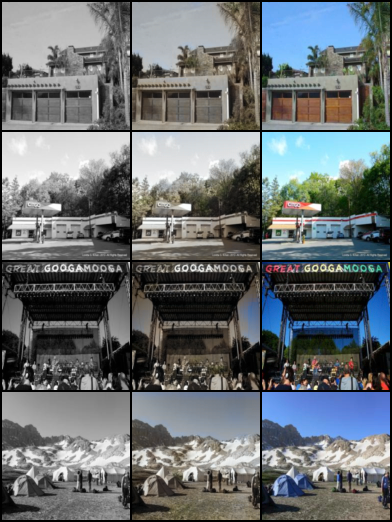
\includegraphics[width=\textwidth]{runs/cnn_baseline/preview_epoch_050.png}
\caption{CNN baseline after 50 epochs ($128\times128$, 4{,}000-image
subset). Colours are faithful but often desaturated relative to ground
truth.}
\label{fig:qual_cnn}
\end{figure*}

\begin{figure*}[!t]
\centering
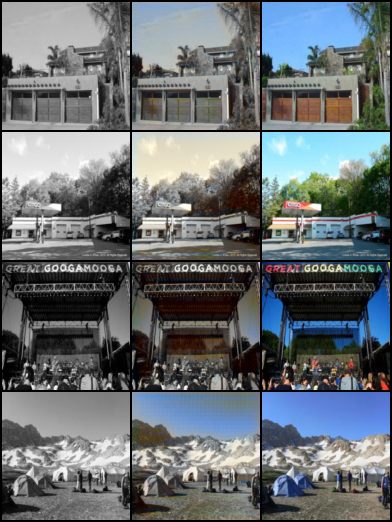
\includegraphics[width=\textwidth]{runs/my_cgan_study/phase2_best/preview_epoch_050.png}
\caption{cGAN (phase-2 best configuration, 50 epochs, $128\times128$).
Sharper than the CNN in high-frequency regions, but still anchored by
the strong L1 term.}
\label{fig:qual_cgan}
\end{figure*}

\begin{figure*}[!t]
\centering
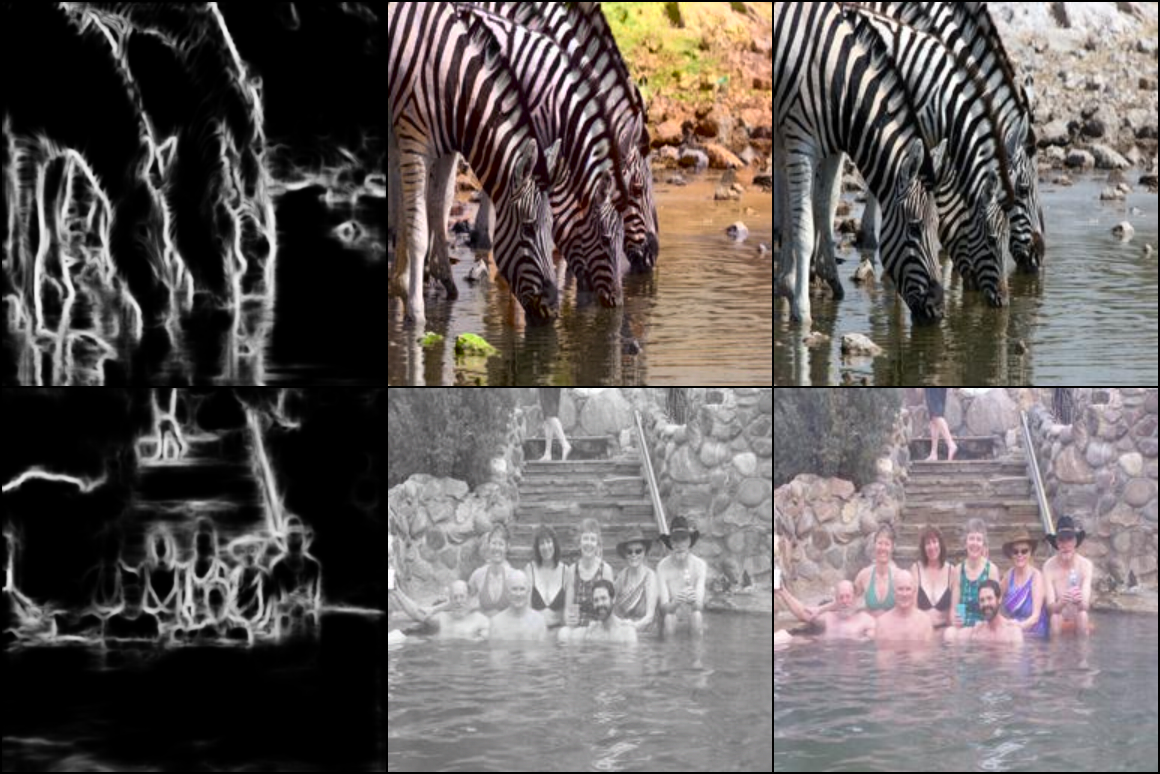
\includegraphics[width=\textwidth]{runs/controlnet_softedge/preview_epoch_010.png}
\caption{ControlNet softedge after 10 epochs ($384\times384$, 8{,}000
images). Structural alignment follows the HED map; chroma is the main
degree of freedom.}
\label{fig:qual_ctrl}
\end{figure*}

\begin{figure*}[!t]
\centering
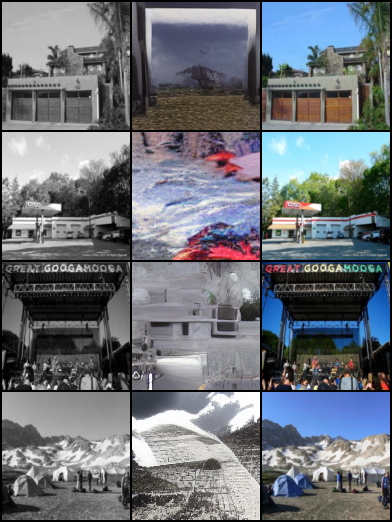
\includegraphics[width=\textwidth]{runs/controlnet_recolor_10ep/preview_epoch_004.png}
\caption{Ablation: ControlNet initialised from \texttt{from\_unet}
with grayscale-as-RGB conditioning (epoch~4 of an interrupted 10-epoch
run at $128\times128$). Middle column shows scene \emph{regeneration}
rather than recolouring---the conditioning signal is too weak for the
frozen SD-1.5 prior.}
\label{fig:qual_ablation}
\end{figure*}

% ============================================================
\section*{Reproducibility}
All code and the pinned dependency list
(\texttt{requirements-controlnet.txt}) are included in the project
repository. The expected hardware bring-up is documented in
\texttt{README.md}.

% ============================================================
\begin{thebibliography}{99}

\bibitem{iizuka2016letthere}
S.~Iizuka, E.~Simo-Serra, and H.~Ishikawa,
``Let there be color! Joint end-to-end learning of global and local image
priors for automatic image colorization with simultaneous classification,''
\emph{ACM Trans.\ Graph.\ (SIGGRAPH)}, 2016.

\bibitem{larsson2016learning}
G.~Larsson, M.~Maire, and G.~Shakhnarovich,
``Learning representations for automatic colorization,''
in \emph{ECCV}, 2016.

\bibitem{zhang2016colorful}
R.~Zhang, P.~Isola, and A.~A. Efros,
``Colorful image colorization,'' in \emph{ECCV}, 2016.

\bibitem{zhang2017realtime}
R.~Zhang, J.-Y. Zhu, P.~Isola, X.~Geng, A.~S. Lin, T.~Yu, and
A.~A. Efros, ``Real-time user-guided image colorization with learned deep
priors,'' \emph{ACM Trans.\ Graph.\ (SIGGRAPH)}, 2017.

\bibitem{isola2017image}
P.~Isola, J.-Y. Zhu, T.~Zhou, and A.~A. Efros,
``Image-to-image translation with conditional adversarial networks,''
in \emph{CVPR}, 2017.

\bibitem{cao2017unsupervised}
Y.~Cao, Z.~Zhou, W.~Zhang, and Y.~Yu,
``Unsupervised diverse colorization via generative adversarial networks,''
in \emph{ECML-PKDD}, 2017.

\bibitem{su2020instance}
J.-W. Su, H.-K. Chu, and J.-B. Huang,
``Instance-aware image colorization,'' in \emph{CVPR}, 2020.

\bibitem{kumar2021colorization}
M.~Kumar, D.~Weissenborn, and N.~Kalchbrenner,
``Colorization transformer,'' in \emph{ICLR}, 2021.

\bibitem{saharia2022palette}
C.~Saharia, W.~Chan, H.~Chang, C.~A. Lee, J.~Ho, T.~Salimans,
D.~Fleet, and M.~Norouzi,
``Palette: Image-to-image diffusion models,'' in \emph{SIGGRAPH}, 2022.

\bibitem{zhang2023adding}
L.~Zhang, A.~Rao, and M.~Agrawala,
``Adding conditional control to text-to-image diffusion models,''
in \emph{ICCV}, 2023.

\bibitem{rombach2022high}
R.~Rombach, A.~Blattmann, D.~Lorenz, P.~Esser, and B.~Ommer,
``High-resolution image synthesis with latent diffusion models,''
in \emph{CVPR}, 2022.

\bibitem{ho2020ddpm}
J.~Ho, A.~Jain, and P.~Abbeel,
``Denoising diffusion probabilistic models,'' in \emph{NeurIPS}, 2020.

\bibitem{xie2015holistically}
S.~Xie and Z.~Tu,
``Holistically-nested edge detection,'' in \emph{ICCV}, 2015.

\bibitem{canny1986computational}
J.~Canny,
``A computational approach to edge detection,''
\emph{IEEE Trans.\ Pattern Anal.\ Mach.\ Intell.}, 1986.

\bibitem{zhou2017places}
B.~Zhou, A.~Lapedriza, A.~Khosla, A.~Oliva, and A.~Torralba,
``Places: A 10 million image database for scene recognition,''
\emph{IEEE Trans.\ Pattern Anal.\ Mach.\ Intell.}, 2017.

\bibitem{mirza2014conditional}
M.~Mirza and S.~Osindero,
``Conditional generative adversarial nets,''
\emph{arXiv preprint arXiv:1411.1784}, 2014.

\bibitem{wang2004image}
Z.~Wang, A.~C. Bovik, H.~R. Sheikh, and E.~P. Simoncelli,
``Image quality assessment: From error visibility to structural similarity,''
\emph{IEEE Trans.\ Image Process.}, vol.~13, no.~4, pp.~600--612, 2004.

\bibitem{lugmayr2022repaint}
A.~Lugmayr, M.~Danelljan, A.~Romero, F.~Yu, R.~Timofte, and L.~Van~Gool,
``RePaint: Inpainting using denoising diffusion probabilistic models,''
in \emph{CVPR}, 2022.

\end{thebibliography}

\end{document}
